\documentclass{standalone}
\usepackage{tikz}
\usepackage{pgfplots}

\pgfplotsset{
    compat=newest,
}

\begin{document}
    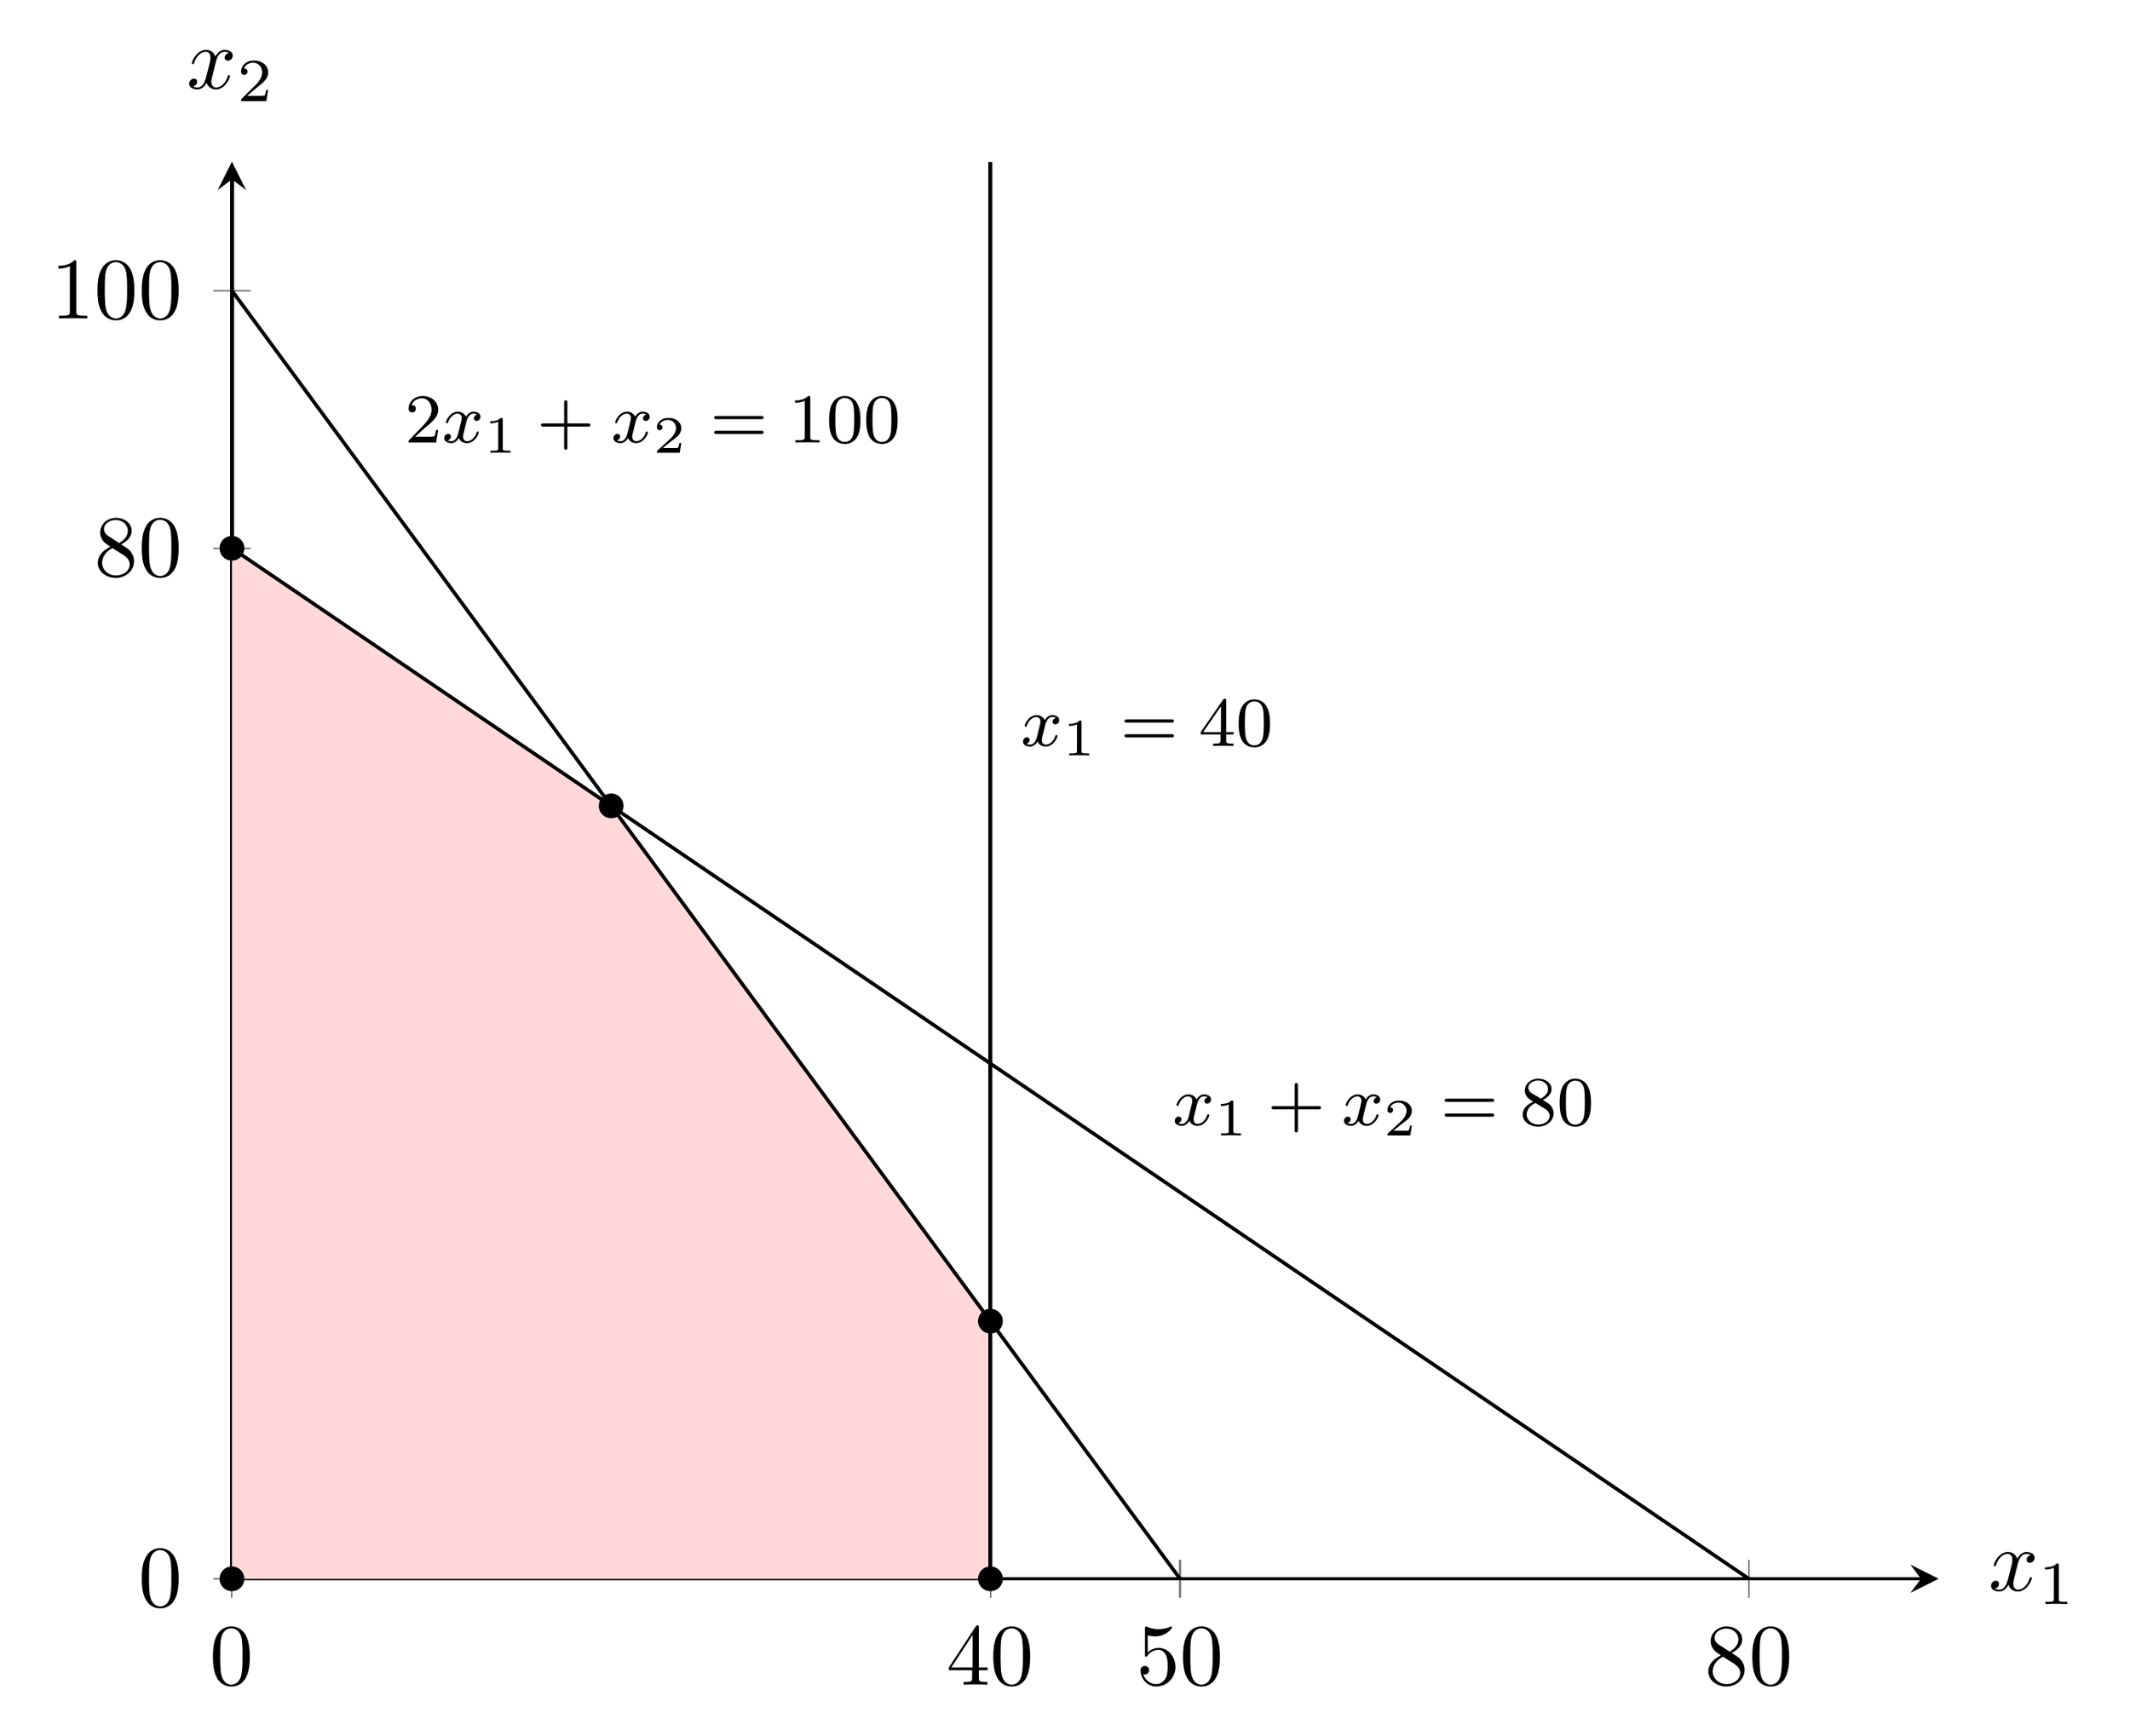
\begin{tikzpicture}[scale=4]
        \begin{axis}[
            axis lines=left,
            ylabel=$x_2$,
            xlabel=$x_1$,
            every axis x label/.style={
                at={(ticklabel* cs:1.1)},
                anchor=east,
            },
            every axis y label/.style={
                at={(ticklabel* cs:1.1)},
                anchor=north,
            },
            xmin=0, ymin=0,
            xmax=90, ymax=110,
            domain=0:80,
            samples=200,
            xtick={0,40,50,80},
            ytick={0,80,100},
            clip=false,
        ]
            \coordinate (A) at (0, 0);
            \coordinate (B) at (40, 0);
            \coordinate (C) at (40, 20);
            \coordinate (D) at (20, 60);
            \coordinate (E) at (0, 80);

            \fill[red!15] (A) -- (B) -- (C) -- (D) -- (E) -- cycle;

            \draw (A) node[circle, fill, inner sep=1pt]{};
            \draw (B) node[circle, fill, inner sep=1pt]{};
            \draw (C) node[circle, fill, inner sep=1pt]{};
            \draw (D) node[circle, fill, inner sep=1pt]{};
            \draw (E) node[circle, fill, inner sep=1pt]{};

            \addplot[domain=0:50] {100 - 2*x} node[pos=0.15, above right]{\footnotesize{$2x_1 + x_2 = 100$}};
            \addplot[] {80 - x} node[pos=0.6, above right]{\footnotesize{$x_1 + x_2 = 80$}};
            \addplot[] coordinates {(40, 0) (40, 110)} node[pos=0.6, right]{\footnotesize{$x_1 = 40$}};
        \end{axis}
    \end{tikzpicture}
\end{document}
